\documentclass{beamer}
\usepackage[utf8]{inputenc}
\usepackage{../UnipdTheme/Padova/beamerthemePadova}
\usepackage{listings}
\lstset{
    language=[LaTeX]Tex,%C++,
    keywordstyle=\color{blue}, %\bfseries,
    basicstyle=\small\ttfamily,
    commentstyle=\color{green}\ttfamily,
    stringstyle=\rmfamily,
    numbers=left,%
    numberstyle=\scriptsize, %\tiny
    stepnumber=1,
    numbersep=8pt,
    showstringspaces=false,
    breaklines=true,
    frameround=ftff,
    frame=single
}
\usepackage{subfig}
\usepackage{wrapfig}
\usepackage{lipsum}
\usepackage[absolute,overlay]{textpos}	

\title{Comandi base}
\subtitle{Immagini, footnote e link}
\author{Davide Polonio \& Marco Zanella}
\date{AA 2017-2018}

\graphicspath{{./res/images/}}

\newenvironment<>{newcommandblock}[1]{%
	\setbeamercolor{block title}{fg=white,bg=blue!75!black}%
	\begin{block}#2{%
		#1%
	}%
}%
{\end{block}}%

\begin{document}

	\maketitle
	\begin{frame}{Inserire immagini nel documento - 1}
	
L'inserimento delle immagini richiede l'utilizzo di un pacchetto, il più
utilizzato è \texttt{graphicx}

\vfill

Il comando per inserire le immagini è \\
\texttt{includegraphics[opzioni]{img\_path}} \\
dove

\begin{itemize}
	\item \texttt{img\_path} indica il percorso dell'immagine
	\item le opzioni che possono essere specificate sono
	\begin{itemize}
		\item width
		\item height
		\item scale
		\item keepaspectratio
	\end{itemize}
\end{itemize}

\end{frame}
	\begin{frame}{Inserimento delle immagini - 2}
	
Le immagini devono essere inserite sfruttando nell'ambiente 
\centerline{
\texttt{\textbackslash{}begin\{figure\}\dots{}\textbackslash{}end\{figure\}}
}

\vfill

Non tutte i formati sono supportati!
\begin{itemize}
	\item PDF
	\item JPG/JPEG
	\item PNG
	\item EPS (nelle versioni recenti)
\end{itemize}

\vfill

È possibile definire un percorso di default per le immagini nel 
\textbf{preambolo} con il comando 
\texttt{\textbackslash{}graphicspath\{\{path/per/le/immagini\}\}}

\end{frame}
	\begin{frame}[fragile]{Inserimento delle immagini - 3}
	
\begin{exampleblock}{Esempio}
	\lstinputlisting{res/examples/esempio.tex}
\end{exampleblock}

\end{frame}
	\begin{frame}{Inserimento delle immagini - 4}
	
\begin{figure}[H]
	\centering
	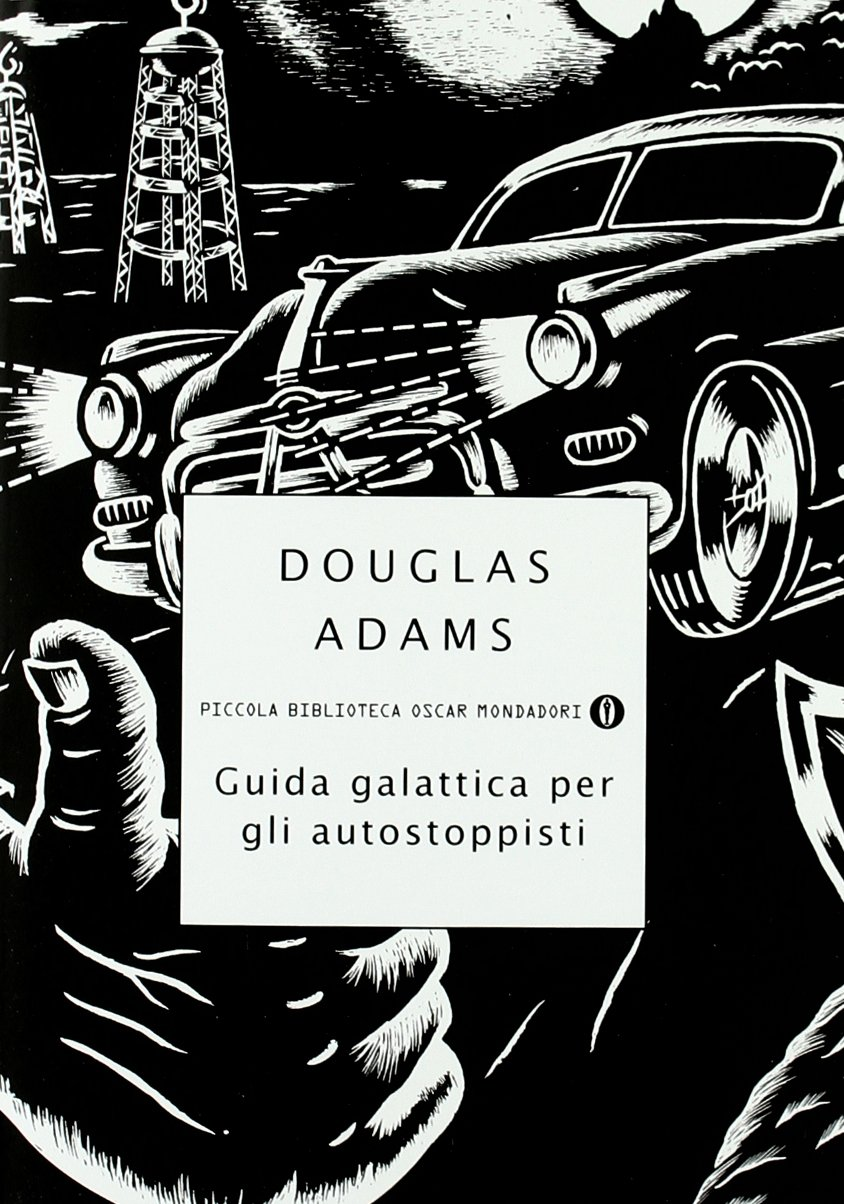
\includegraphics[scale=0.10]{immagine}
	\caption{Didascalia dell'immagine}
\end{figure}

\end{frame}
	\begin{frame}{Affiancare le immagini - 1}

\begin{itemize}
	\item Per affiancare più immagini consigliamo di utilizzare il pacchetto 
	\texttt{subfig}
	\item Si utilizza lo stesso ambiente 
	\texttt{\textbackslash{}begin\{figure\}\dots{}\textbackslash{}end\{figure\}}
	e le stesse regole di prima
	\item Per mandare a capo un immagine si utilizza il comando 
	\texttt{\textbackslash{}\textbackslash{}} mentre per definire la spaziatura 
	orizzontale è possibile specificare la distanza con 
	\texttt{\textbackslash{}hspace} oppure utilizzare 
	\texttt{\textbackslash{}hfill}
	\item Per specificare ogni immagine viene utilizzato il comando
	\texttt{\textbackslash{}subfloat}
\end{itemize}

\end{frame}

	\begin{frame}[fragile]{Affiancare le immagini - 2}

\begin{exampleblock}{Esempio}
	\lstinputlisting{res/examples/esempio4immagini.tex}
\end{exampleblock}

\end{frame}
	\begin{frame}{Affiancare le immagini - 3}

\begin{figure}[H]
	\centering
	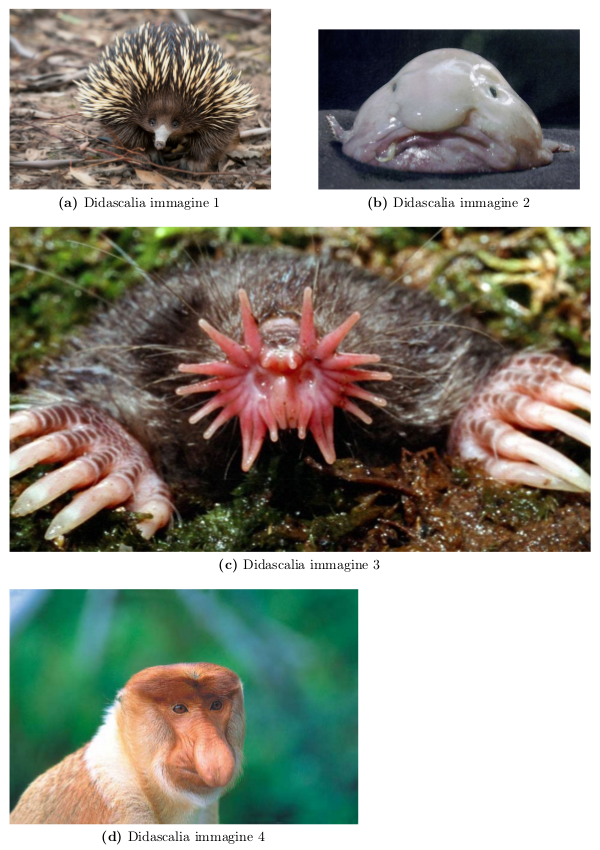
\includegraphics[scale=0.34]{img4}
\end{figure}

\end{frame}
	\begin{frame}{Affiancare immagini e testo - 1}

\begin{itemize}
	\item Per affiancare immagini e testo consigliamo di utilizzare il pacchetto 
	\texttt{wrapfig}
	\item L'ambiente da utilizzare cambia ed è
	\texttt{\textbackslash{}begin\{wrapfigure\}\{pos\}\{dim\}
	\dots{}\textbackslash{}end\{wrapfigure\}} dove
	\begin{itemize}
		\item \textbf{pos} può essere \textbf{r}(immagine affiancata a destra)
		o \textbf{l} (affiancata a sinistra)
		\item \textbf{dim} indica di quanto l'immagine si affianca al testo
	\end{itemize}
\end{itemize}

\end{frame}

	\begin{frame}[fragile]{Affiancare immagini e testo - 2}

\begin{exampleblock}{Esempio}
	\lstinputlisting{res/examples/esempiotestoafianco.tex}
\end{exampleblock}

\end{frame}
	\begin{frame}{Affiancare immagini e testo - 3}

Lorem ipsum dolor sit amet, consectetur adipiscing elit. In bibendum vel nulla eu egestas. Nam sit amet egestas urna. Proin eu arcu augue. Praesent
\begin{wrapfigure}{r}{5cm}
    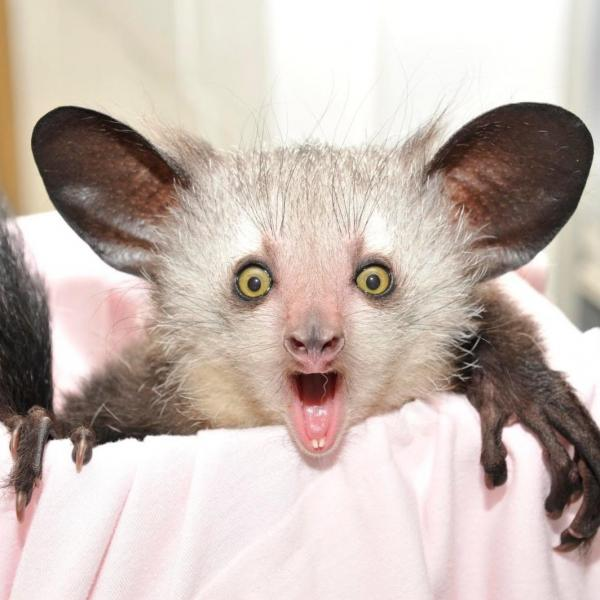
\includegraphics[scale=0.21]{immagineafianco}
    \caption{Didascalia dell'immagine}
\end{wrapfigure} 
tincidunt ullamcorper lectus vel egestas. Fusce ac ultricies augue. In id interdum libero. Sed lobortis libero id sapien aliquet laoreet. Etiam accumsan nunc sed est facilisis, vitae condimentum ex blandit. Praesent lacinia ligula purus, id interdum ex dapibus non. Donec consequat porttitor felis eu pretium. In vestibulum mollis fringilla. Nam suscipit dictum eros sit amet porttitor.

\end{frame}
	\begin{frame}{Esercizi}

\begin{block}{Esercizio 1}
Creare un documento \texttt{book} che contenga un'immagine
\end{block}

\begin{block}{Esercizio 2}
Estendere l'esercizio 1 affiancando il testo all'immagine
\end{block}

\begin{block}{Esercizio 3}
Mettere nel documento l'immagine che trovate in \url{www.google.it} in modo che
venga visualizzata interamente e più grande possibile
\end{block}

\end{frame}
	\begin{frame}[fragile]{Soluzione esercizio 3}

\begin{block}{Soluzione}
\begin{lstlisting}
\documentclass{article}
\usepackage[a4paper,margin=1in,landscape]{geometry}
\usepackage{graphicx}
\begin{document}

\begin{figure}
	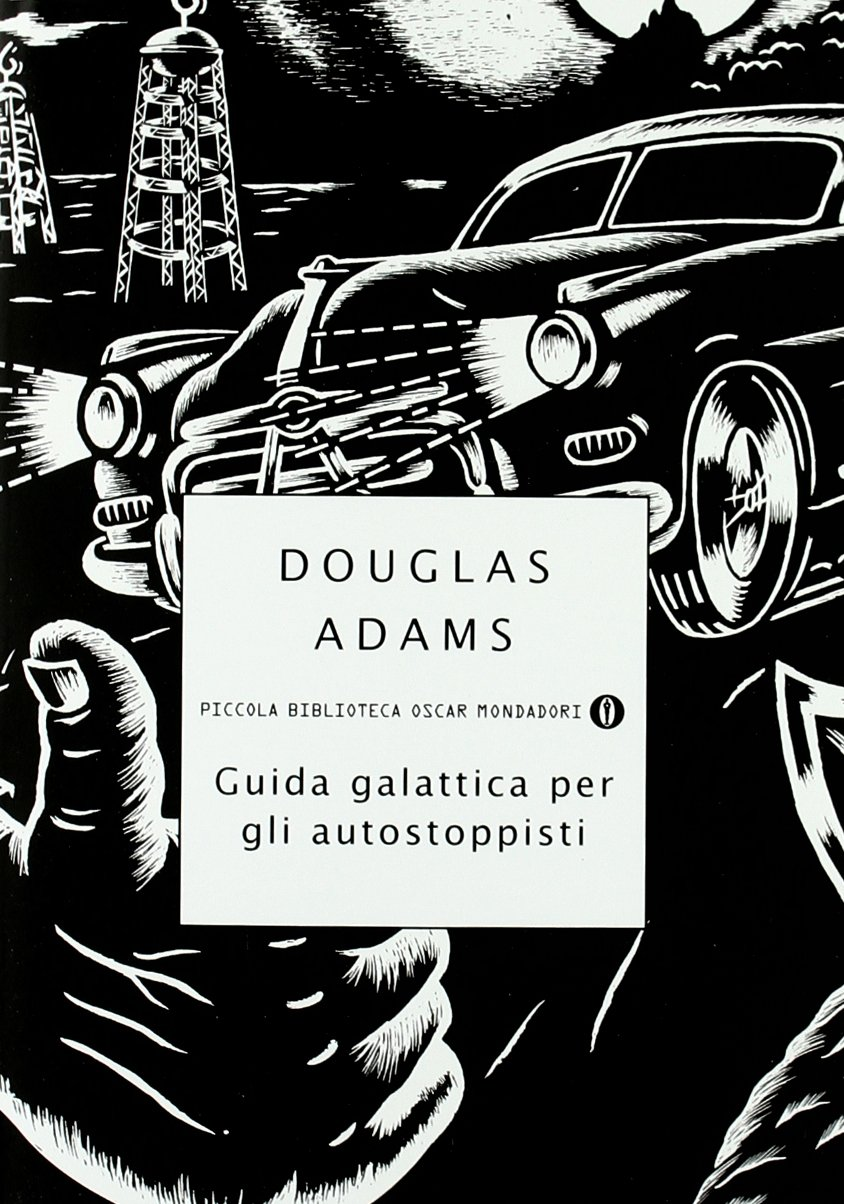
\includegraphics[width=\textwidth]{immagine}
\end{figure}

\end{document}
\end{lstlisting}
\end{block}

\end{frame}
	\begin{frame}{Note a piè di pagina}

Per inserire le note a piè di pagina è possibile utilizzare il comando 
\texttt{footnote}

\vfill

\LaTeX{} si occupa in automatico di posizionamento e della numerazione

\vfill

\begin{exampleblock}{Esempio}
\dots{}In questo testo c'è una precisazione\textbackslash{}footnote
\{Inserita qui\}\dots{}
\end{exampleblock}

\end{frame}
	\begin{frame}{Collegamenti nel documento - 1}

È possibile creare dei collegamenti ipertestuali in un documento usando i 
comandi \texttt{label} e \texttt{ref} specificando un identificativo per il 
riferimento

\vfill

È possibile anche riferirsi semplicemente alla pagina in cui è presente un
certo elemento usando il comando \texttt{pageref} invece che \texttt{ref}

\vfill

È buona norma utilizzare degli identificativi esplicativi che indichino a cosa
ci si riferisce, anche antecedendo all'identificatore un prefisso
\begin{description}
	\item [fig:] per le figure
	\item [tab:] per le tabelle
	\item [sec:] per una sezione
\end{description}

\end{frame}
	\begin{frame}[fragile]{Collegamenti nel documento - 2}

\begin{exampleblock}{Esempio}
	\lstinputlisting{res/examples/esempiolink}
\end{exampleblock}

\end{frame}
	\begin{frame}{Indirizzi Web}

Per inserire URL nel testo è consigliato l'utilizzo del pacchetto 
\texttt{hyperref} che mette a disposizione due comandi 
\begin{itemize}
	\item \textbf{\textbackslash{}url\{indirizzo\}} per mostrare un certo
	indirizzo con il formato monospace
	\item \textbf{\textbackslash{}href\{indirizzo\}\{testo\}} che non mostrerà
	l'indirizzo ma il testo indicato
\end{itemize}

\vfill

La prima modalità è utile per i documenti cartacei, la seconda per quelli per
la fruizione in via digitale

\end{frame}
	\begin{frame}[fragile]{E-Mail}

Il pacchetto \texttt{hyperref} non prevede alcun comando per l'inserimento di
indirizzi di posta elettronica ma è spesso utile crearne uno da aggiungere nel
preambolo

\begin{lstlisting}
\newcommand{\mail}[1]{\href{mailto:#1}
{\texttt{#1}}}
\end{lstlisting}

\begin{figure}
	\centering
	
\includegraphics[scale=0.25]{res/images/email}
\end{figure}

\end{frame}
	\begin{frame}{Esercizi}

\begin{block}{Esercizio 4}

creare un documento che contenga un elenco puntato con
\begin{itemize}
	\item almeno un riferimento ad un'immagine
	\item almeno un riferimento ad una tabella
	\item almeno un riferimento ad una sezione
	\item almeno un URL
\end{itemize}

\end{block}

\end{frame}
	\begin{frame}[fragile]{Soluzione esercizio 4}

\begin{block}{Soluzione incompleta}
\begin{lstlisting}
\section{Sezione}\label{sec:sezione}
\begin{figure}
	...
	\label{fig:immagine}
\end{figure}
\begin{table}[h!]
...
\label{tab:tabella}
\end{table}
\begin{itemize}
	\item Sezione~\ref{sec:sezione}
	\item Tabella~\ref{tab:tabella}
	\item Immagine~\ref{fig:immagine}
	\item \url{www.google.it}
\end{itemize}
\end{lstlisting}
\end{block}

\end{frame}

\end{document}
